\chapter{Green 算符与预解式 (Green Operator and Resolvent)}\label{ch:green}

在前面几章中，我们用与时间有关的 (time-dependent) 框架建立了
M\o ller 算符 $\Omega_\pm$、$S$ 算符以及散射截面之间的关系。
本章开始，我们将转向\emph{与时间无关的} (time-independent) 表述。
其核心目的是：
\begin{itemize}
  \item 由一个给定的相互作用势 $V$ 出发，直接计算 $S$ 矩阵元、散射振幅以及散射截面；
  \item 引入两个在与时间无关表述中起决定性作用的算符：
        \emph{Green 算符 (Green's operator)}，又称\emph{预解式 (resolvent)} $G(z)$；
        以及 \emph{$T$ 算符} (transition operator)。
\end{itemize}
为简单起见，我们仅考虑单粒子情形 (即把两体问题约化到质心系后的有效单体问题)，
并将所得结果向两粒子情形作直接的推广。

\section{Green 算符的定义}

设 Hamiltonian 形如
\begin{equation}
  H = H_0 + V,\qquad H_0 = \frac{\bm{P}^2}{2m},
\end{equation}
其中 $H_0$ 为自由 Hamiltonian，$V$ 为局域势。
对应的 \emph{Green 算符} 或 \emph{resolvent} 定义为
\begin{equation}\label{eq:green-def}
  G(z) \equiv (z - H)^{-1},\qquad
  G_0(z) \equiv (z - H_0)^{-1},\qquad z\in\C.
\end{equation}

\begin{remark}[算符层面的意义]
若逆算符 $(z-H_0)^{-1}$ 在整个 Hilbert 空间 $\Hilb$ 上良好定义，
则有算符等式 $(z-H_0)\,G_0(z)=\mathbf{1}$。在坐标表象下取矩阵元，
利用 $\matel{\bm x}{H_0}{\bm x'} = -\frac{\nabla^2}{2m}\,\delta_3(\bm x-\bm x')$，
可得
\begin{equation}\label{eq:G0-coordinate-greens-fn}
  \left(\frac{\nabla^2}{2m} + z\right)\matel{\bm x}{G_0(z)}{\bm x'}
  = \delta_3(\bm x - \bm x').
\end{equation}
所以 $G_0(z)$ 在坐标表象下的矩阵元
$\matel{\bm x}{G_0(z)}{\bm x'}$
正是微分算符 $\frac{\nabla^2}{2m}+z$ 的 \emph{Green 函数}。
对完整的 $G(z)$，类似地 $\matel{\bm x}{G(z)}{\bm x'}$
是 $\frac{\nabla^2}{2m}-V(\bm x)+z$ 的 Green 函数。
这正是 \emph{Green 算符} 这一名称的来历。
\end{remark}

\begin{remark}[定义域问题]
并非对所有 $z\in\C$，$G(z)$ 都在整个 $\Hilb$ 上有定义：
若 $E_n$ 为 $H$ 的本征值、$\ket{n}\in\Hilb$ 为对应的本征矢，
那么 $(H-E_n)\ket{n}=0$，即 $z-H$ 在 $z=E_n$ 处不可逆，
$G(E_n)$ 没有定义，或更确切地说其定义域只是 $\Hilb$ 的一个真子集。
所以 $G(z)$ 的奇异结构记录着 $H$ 的谱。
\end{remark}

\section{$G(z)$ 的解析结构与谱}

\subsection{纯分立谱情形}

先假设 $H$ 只有分立 (point) 谱，记本征值为 $\{E_n\}$，
对应归一化本征矢 $\ket{n}$，$H\ket{n}=E_n\ket{n}$，
$\sum_n\ket{n}\bra{n}=\mathbf 1$。利用谱分解
\begin{equation}\label{eq:G-spectral-discrete}
  G(z) = (z-H)^{-1} = \sum_n \frac{\ket{n}\bra{n}}{z-E_n}.
\end{equation}
由此立刻得到下述性质：
\begin{itemize}
  \item 若 $z\neq E_n$ ($\forall n$)，则 $G(z)$ 在整个 $\Hilb$ 上有定义：
        $\forall \ket{\chi}\in\Hilb,\ G(z)\ket{\chi}\in\Hilb$；
  \item 对 $\forall \ket{\chi},\ket{\psi}\in\Hilb$，矩阵元
        \begin{equation}
          \matel{\chi}{G(z)}{\psi}
          = \sum_n \frac{\inn{\chi}{n}\inn{n}{\psi}}{z-E_n}
        \end{equation}
        是 $z$ 在 $\C\setminus\{E_n\}$ 上的解析函数。
        我们称 $G(z)$ 是关于 $z$ 的\emph{解析的算符函数}；
  \item 在 $z=E_n$ 处，$G(z)$ 有简单极点 (simple pole)，
        其留数为对应的投影算符
        \begin{equation}
          \Res_{z=E_n} G(z) = \ket{n}\bra{n}.
        \end{equation}
\end{itemize}
所以，知道了 $G(z)$ 就等于知道了 $H$ 的本征值问题的解：
\begin{center}
\fbox{$G(z)$ 的极点位置 $\longrightarrow$ 本征值；\quad
留数 $\longrightarrow$ 本征态投影算符。}
\end{center}

\subsection{连续谱情形：割线的出现}

当 $H$ 拥有连续谱时，对应散射 ``本征态''——这些 ``态'' 是
\emph{广义} (improper) 的、不可归一化的 ket。
以 $H_0=\bm P^2/2m$ 为例，在动量–角动量基 $\ket{E,\ell,m}$ 下，
$H_0\ket{E,\ell,m}=E\ket{E,\ell,m}$，$E\in(0,\infty)$，
$\sum_{\ell,m}\int_0^\infty\rmd E\,\ket{E,\ell,m}\bra{E,\ell,m}=\mathbf 1$.
$G_0$ 在该基下的谱表示为
\begin{equation}\label{eq:G0-spectral}
  G_0(z) = \sum_{\ell,m}\int_0^\infty \rmd E\,
           \frac{\ket{E,\ell,m}\bra{E,\ell,m}}{z-E}.
\end{equation}
取任一对 $\ket{\chi},\ket{\psi}\in\Hilb$，
\begin{equation}
  \matel{\chi}{G_0(z)}{\psi}
  = \sum_{\ell,m}\int_0^\infty \rmd E\,
    \frac{\inn{\chi}{E,\ell,m}\inn{E,\ell,m}{\psi}}{z-E}.
\end{equation}
\begin{itemize}
  \item 当 $z\notin (0,\infty)$ 时，被积函数无奇点，积分收敛，
        $\matel{\chi}{G_0(z)}{\psi}$ 关于 $z$ 解析；
  \item 但当 $z\in(0,\infty)$ 时，$z-E$ 在积分路径上有零点，
        积分作为 $z$ 的函数在正实轴上不连续——出现\emph{割线}。
\end{itemize}

\subsubsection*{割线两边的不连续性}

把 $z$ 取到正实轴的上下两侧 $z=E_0\pm\rmi 0^+$ ($E_0>0$)，
两式相减利用 Sokhotski--Plemelj 公式
$\frac{1}{x-\rmi 0^+}-\frac{1}{x+\rmi 0^+}=2\pi\rmi\,\delta(x)$,
\begin{align}
  \matel{\chi}{G_0(E_0+\rmi 0^+)}{\psi}
  -\matel{\chi}{G_0(E_0-\rmi 0^+)}{\psi}
  &= \sum_{\ell,m}\int_0^\infty \rmd E\,
     \inn{\chi}{E,\ell,m}\inn{E,\ell,m}{\psi}\notag\\
  &\quad\times\left(\frac{1}{E_0-E+\rmi 0^+}-\frac{1}{E_0-E-\rmi 0^+}\right)\notag\\
  &= -2\pi\rmi\sum_{\ell,m}\inn{\chi}{E_0,\ell,m}\inn{E_0,\ell,m}{\psi}.
\end{align}
所以 $G_0(z)$ 在 $z\in(0,\infty)$ 上有割线，
不连续性恰为
\begin{equation}\label{eq:G0-discontinuity}
  G_0(E_0+\rmi 0^+) - G_0(E_0-\rmi 0^+)
  = -2\pi\rmi\sum_{\ell,m}\ket{E_0,\ell,m}\bra{E_0,\ell,m}.
\end{equation}
即\emph{割线的不连续性正是 $H_0$ 在该能量处的连续谱投影算符 ($\times -2\pi\rmi$)}。

\subsection{一般情形}

更一般地，若 $H$ 既有分立束缚态谱 $E_1,E_2,\dots<0$，
又有连续散射谱 $E>0$，则 $G(z)$ 的解析结构可总结如下：
\begin{itemize}
  \item $G(z)$ 在 $\C\setminus\{E_n\}\setminus(0,\infty)$ 上解析；
  \item 在 $z=E_1,E_2,\dots$ ($<0$) 处有简单极点；
  \item 在 $z\in(0,\infty)$ 上有割线；
  \item 知道了 $G(z)$ 的解析结构，等价于知道了 $H$ 的整个本征值问题的解。
\end{itemize}

\begin{proposition}[厄米性质带来的对称性]
由于 $H=H^\dagger$ 厄米，由 $G(z)=(z-H)^{-1}$ 取共轭得
\begin{equation}\label{eq:G-conjugation}
  G(z^*) = [G(z)]^\dagger,
\end{equation}
对 $G_0(z)$ 同样成立。这意味着 $G(z)$ 的实轴上下值互为厄米共轭，
割线两边的奇异部分互相联系。
\end{proposition}

\subsection{推迟与超前 Green 算符}

把 $z$ 从复平面贴到实轴正侧（散射能量 $E>0$），定义
\begin{equation}\label{eq:Gpm-def}
  G^\pm(E) \equiv \lim_{\epsilon\to 0^+} G(E\pm\rmi\epsilon),
  \qquad
  G_0^\pm(E) \equiv \lim_{\epsilon\to 0^+} G_0(E\pm\rmi\epsilon).
\end{equation}
$G^+$ 称为\emph{推迟 (retarded)} Green 算符，
$G^-$ 称为\emph{超前 (advanced)} Green 算符。
两者之差由式 \eqref{eq:G0-discontinuity} 给出：
$G_0^+ - G_0^-$ 把任意态投影到能壳 $E$ 上的所有自由
``本征态'' 上，并乘以 $-2\pi\rmi$。
推迟/超前 Green 算符在与时间无关散射框架以及时间依赖框架中，
分别对应于 $\Omega_+$ 与 $\Omega_-$，这一关系将在第 \ref{sec:moller} 节展开。

\section{自由 Green 算符的具体表示}

\subsection{动量表象}

由于 $H_0=\bm P^2/2m$ 在动量表象下是乘法算符，
\begin{equation}\label{eq:G0-momentum}
  G_0(z)\ket{\bm p} = (z-H_0)^{-1}\ket{\bm p}
  = \frac{1}{z-E_p}\ket{\bm p},\qquad
  E_p \equiv \frac{p^2}{2m}.
\end{equation}
即 $G_0(z)$ 在动量表象下完全对角，本征值为 $1/(z-E_p)$。

\subsection{坐标表象下的 3D 自由 Green 函数}

由 \eqref{eq:G0-coordinate-greens-fn} 出发，需要解
$\bigl(\nabla^2/(2m)+z\bigr) G_0(\bm x,\bm x';z)=\delta_3(\bm x-\bm x')$。
设 $z=E\pm\rmi\epsilon$，并令 $k^2=2mE$，则方程变为 Helmholtz 方程
$(\nabla^2+k^2)\,2m\,G_0^\pm(\bm x,\bm x';E)=2m\,\delta_3(\bm x-\bm x')$.
利用平面波展开
$\delta_3(\bm x-\bm x')=\int\frac{\rmd^3 p}{(2\pi)^3}\,\rme^{\rmi\bm p\cdot(\bm x-\bm x')}$
以及 \eqref{eq:G0-momentum}，
\begin{align}
  G_0^\pm(\bm x,\bm x';E)
  &= \matel{\bm x}{G_0(E\pm\rmi 0^+)}{\bm x'}\notag\\
  &= \int\frac{\rmd^3 p}{(2\pi)^3}\,
     \frac{\rme^{\rmi\bm p\cdot(\bm x-\bm x')}}{E\pm\rmi 0^+ - p^2/(2m)}\notag\\
  &= -\frac{2m}{(2\pi)^3}\int\rmd^3 p\,
     \frac{\rme^{\rmi\bm p\cdot(\bm x-\bm x')}}{p^2-k^2\mp\rmi 0^+}.
\end{align}
此积分用留数定理（绕过实轴上的极点 $p=\pm k$）可计算为闭式
\begin{equation}\label{eq:G0-3d-coord}
  \boxed{\,G_0^\pm(\bm x,\bm x';E)
  = -\frac{m}{2\pi}\,\frac{\rme^{\pm\rmi k|\bm x-\bm x'|}}{|\bm x-\bm x'|},\qquad
  k=\sqrt{2mE}>0.\,}
\end{equation}
$G_0^+$ 对应外向球面波 (outgoing)，
$G_0^-$ 对应内向球面波 (incoming)。
正是这一不连续性将后面的 Lippmann--Schwinger 方程的两支
$\ket{\phi\pm}$ 区分开来。

\section{Lippmann--Schwinger 方程：联系 $G$ 与 $G_0$}

实际中我们想由 \emph{已知} 算符 $G_0$ 及势 $V$ 解出 $G(z)$。
利用一般恒等式
\begin{equation}\label{eq:operator-identity}
  A^{-1} = B^{-1} + B^{-1}(B-A)A^{-1},
\end{equation}
对其中两种取法分别赋值：
\begin{itemize}
  \item 取 $A=z-H,\ B=z-H_0$，则 $B-A=V$，$A^{-1}=G$，$B^{-1}=G_0$；
  \item 取 $A=z-H_0,\ B=z-H$，则 $B-A=-V$，与上式互换 $G,G_0$。
\end{itemize}
分别代入 \eqref{eq:operator-identity}，得到\emph{第二预解式恒等式}
(second resolvent identity，又称 Dyson 恒等式)：
\begin{equation}\label{eq:LS-G}
  \boxed{\,G(z) = G_0(z) + G_0(z)\,V\,G(z)
                 = G_0(z) + G(z)\,V\,G_0(z).\,}
\end{equation}
此即 $G(z)$ 的 \emph{resolvent equation}，
也称作 $G(z)$ 的 \emph{Lippmann--Schwinger 方程}。
它把未知的全 Green 算符 $G$ 与已知的 $G_0$ 通过势 $V$ 联系起来。
由此还可立即读出
\begin{equation}\label{eq:G-minus-G0}
  G(z) - G_0(z) = G_0(z)\,V\,G(z) = G(z)\,V\,G_0(z).
\end{equation}

如果 $V$ 足够弱，可以把 \eqref{eq:LS-G} 迭代展开，得到 Born 级数
$G = G_0 + G_0 V G_0 + G_0 V G_0 V G_0 + \cdots$，
我们将在下一章详细讨论。

\section{$T$ 算符}\label{sec:Tmat}

为了把 $G$ 中含 ``一次'' 势的部分分离出来，引入 \emph{$T$ 算符}
(transition operator)：
\begin{equation}\label{eq:T-def}
  T(z) \equiv V + V\,G(z)\,V.
\end{equation}

\begin{proposition}[$T$ 算符的解析性]
$T(z)$ 关于 $z$ 的解析性由 $G(z)$ 决定：
\begin{itemize}
  \item 当 $z$ 不属于 $H$ 的谱时，$T(z)$ 解析；
  \item 在 $H$ 的分立本征值处 $T(z)$ 有极点，
        在 $H$ 的连续谱上 $T(z)$ 有割线；
  \item 类似 $G(z)$，$T(z^*)=[T(z)]^\dagger$。
\end{itemize}
\end{proposition}

\subsection{$T$, $G$, $G_0$ 三者的代数关系}

由定义 \eqref{eq:T-def} 与 Lippmann--Schwinger 方程 \eqref{eq:LS-G}：
\begin{equation}\label{eq:G0T-equals-GV}
  G_0(z)\,T(z) = G_0(V + VGV) = (G_0 + G_0 V G)V = G(z)\,V,
\end{equation}
\begin{equation}\label{eq:TG0-equals-VG}
  T(z)\,G_0(z) = (V + VGV)G_0 = V(G_0 + G V G_0) = V\,G(z).
\end{equation}
利用 \eqref{eq:G0T-equals-GV} 把 \eqref{eq:LS-G} 中的 $VG$ 替换：
\begin{equation}\label{eq:G-via-T}
  \boxed{\,G(z) = G_0(z) + G_0(z)\,T(z)\,G_0(z).\,}
\end{equation}
所以 ``有了 $T(z)$ 就等同于得到了 $G(z)$''，反之亦然。
进一步利用 \eqref{eq:TG0-equals-VG} 写出 $T$ 自身满足的方程：
\begin{equation}\label{eq:LS-T}
  \boxed{\,T(z) = V + V\,G_0(z)\,T(z) = V + T(z)\,G_0(z)\,V.\,}
\end{equation}
此即 \emph{$T(z)$ 的 Lippmann--Schwinger 方程}。
若 $V$ 足够弱，可迭代得到形式解
\begin{equation}\label{eq:T-Born}
  T = V + V G_0 V + V (G_0 V)^2 + V (G_0 V)^3 + \cdots
\end{equation}

\section{Green 算符、$T$ 算符与 M\o ller 算符、$S$ 算符及散射态的关系}\label{sec:moller}

下面给出在与时间无关表述中，$G$ 和 $T$ 与之前 (与时间有关) 表述中的
M\o ller 算符 $\Omega_\pm$、$S$ 算符之间的具体联系。

\subsection{由 M\o ller 算符出发}

回顾入射渐近态 $\ket{\psi_{\rm in}}=\ket{\phi}$ (假设已归一化)，
对应于 $t=0$ 时刻的物理态
\begin{equation}
  \ket{\psi} = \Omega_+\ket{\psi_{\rm in}} = \Omega_+\ket\phi
  \equiv \ket{\phi+}.
\end{equation}
同样，对渐近出射态 $\ket{\psi_{\rm out}}=\ket\phi$，
\begin{equation}
  \ket{\psi} = \Omega_-\ket{\psi_{\rm out}} = \Omega_-\ket\phi
  \equiv \ket{\phi-}.
\end{equation}
M\o ller 算符的积分表示为 (利用
$\bigl(U^\dagger(t)U_0(t)\bigr)' = \rmi U^\dagger(t)\,V\,U_0(t)$,
其中 $U(t)=\rme^{-\rmi Ht}$，$U_0(t)=\rme^{-\rmi H_0 t}$)：
\begin{equation}\label{eq:Omega-integral}
  \Omega_\pm = \lim_{t\to\mp\infty} U^\dagger(t)U_0(t)
  = \rmi\int_0^{\mp\infty}\rmd\tau\, U^\dagger(\tau)\,V\,U_0(\tau) + 1.
\end{equation}
对 $\Omega_-$ 取 $t\to+\infty$，作用到 $\ket\phi$：
\begin{equation}\label{eq:phi-minus-integral}
  \ket{\phi-} = \ket\phi + \rmi\int_0^{+\infty}\rmd\tau\,
                    U^\dagger(\tau)\,V\,U_0(\tau)\ket\phi.
\end{equation}
之前已经说明此积分为绝对收敛。

\subsection{绝热引入}

对一个绝对收敛的积分 $\int_0^\infty\rmd\tau\,\ket{\psi_\tau}$，下式成立：
\begin{equation}
  \int_0^\infty\rmd\tau\,\ket{\psi_\tau}
  = \lim_{\epsilon\downarrow 0}\int_0^\infty\rmd\tau\,
    \rme^{-\epsilon\tau}\ket{\psi_\tau}.
\end{equation}
所以 \eqref{eq:phi-minus-integral} 可写为
\begin{equation}\label{eq:phi-minus-adiabatic}
  \ket{\phi-} = \Omega_-\ket\phi
  = \ket\phi + \rmi\lim_{\epsilon\downarrow 0}
    \int_0^{\infty}\rmd\tau\,\rme^{-\epsilon\tau}\,
    U^\dagger(\tau)\,V\,U_0(\tau)\ket\phi.
\end{equation}
同理
\begin{equation}\label{eq:phi-plus-adiabatic}
  \ket{\phi+} = \Omega_+\ket\phi
  = \ket\phi + \rmi\lim_{\epsilon\downarrow 0}
    \int_0^{-\infty}\rmd\tau\,\rme^{+\epsilon\tau}\,
    U^\dagger(\tau)\,V\,U_0(\tau)\ket\phi.
\end{equation}
\begin{remark}
\eqref{eq:phi-minus-adiabatic} 之所以成立：
\begin{itemize}
  \item 用到了 \eqref{eq:phi-minus-integral} 在 proper 态上积分足够收敛，
        因为 proper 波包在 $t\to\pm\infty$ 会弥散，振幅 $\to 0$；
  \item $\rme^{-\epsilon\tau}$ 因子保证当我们把 $\ket\phi$ 替换成 \emph{improper} 态
        (例如 $\ket{\bm p}$) 时积分仍收敛；
  \item 物理图像是把 $V$ 替换成 $V\rme^{-\epsilon|\tau|}$
        (\emph{绝热近似}, adiabatic approximation)。
        当 $|\tau|\to\infty$ 两粒子远离，相互作用趋于零；
        而对任意轨道 (有限作用时间)，$\epsilon$ 取得足够小后，
        $V$ 与 $V\rme^{-\epsilon|\tau|}$ 在所关心的时间窗内几乎没有差别。
\end{itemize}
\end{remark}

\subsection{插入完备基：$\Omega_\pm$ 化为 $G$ 的形式}

把 $\ket\phi$ 用动量本征矢展开，
$\ket\phi = \int\rmd^3 p\,\ket{\bm p}\inn{\bm p}{\phi}$，
代入 \eqref{eq:phi-minus-adiabatic}：
\begin{align}
  \ket{\phi-}
  &= \ket\phi + \rmi\lim_{\epsilon\downarrow 0}\int\rmd^3 p\int_0^{\infty}\rmd\tau\,
     \rme^{-\epsilon\tau}\,U^\dagger(\tau)\,V\,U_0(\tau)\ket{\bm p}\inn{\bm p}{\phi}\notag\\
  &= \ket\phi + \rmi\lim_{\epsilon\downarrow 0}\int\rmd^3 p\int_0^{\infty}\rmd\tau\,
     \rme^{-\epsilon\tau}\,\rme^{\rmi H\tau}\,V\,
     \rme^{-\rmi E_p \tau}\ket{\bm p}\inn{\bm p}{\phi}\notag\\
  &= \ket\phi + \rmi\lim_{\epsilon\downarrow 0}\int\rmd^3 p\,
     \frac{-\rmi}{E_p - H -\rmi\epsilon}\,V\,\ket{\bm p}\inn{\bm p}{\phi}\notag\\
  &= \ket\phi + \lim_{\epsilon\downarrow 0}\int\rmd^3 p\,
     G(E_p-\rmi\epsilon)\,V\,\ket{\bm p}\inn{\bm p}{\phi}.\label{eq:phi-minus-G}
\end{align}
中间一步用了 $\int_0^\infty\rmd\tau\,\rme^{\rmi(E_p-H+\rmi\epsilon)\tau}
=-\rmi/(E_p-H+\rmi\epsilon)$ 反号给出 $-\rmi/(E_p-H-\rmi\epsilon)$
(注意 $\rmi$ 因子整理)。
同理由 \eqref{eq:phi-plus-adiabatic}：
\begin{equation}\label{eq:phi-plus-G}
  \ket{\phi+} = \ket\phi + \lim_{\epsilon\downarrow 0}\int\rmd^3 p\,
     G(E_p+\rmi\epsilon)\,V\,\ket{\bm p}\inn{\bm p}{\phi}.
\end{equation}

\begin{remark}
\eqref{eq:phi-plus-G} 与 \eqref{eq:phi-minus-G} 中
$\rmi\epsilon$ 前的符号与 $\Omega_\pm$ 下标的符号一致：
$\Omega_+\to G^+$，$\Omega_-\to G^-$。
\end{remark}

利用 \eqref{eq:G0T-equals-GV}，即 $GV=G_0 T$，可将 \eqref{eq:phi-plus-G}--\eqref{eq:phi-minus-G}
统一写成
\begin{align}
  \ket{\phi\pm} \equiv \Omega_\pm\ket\phi
  &= \ket\phi + \lim_{\epsilon\downarrow 0}\int\rmd^3 p\,
     G(E_p\pm\rmi\epsilon)\,V\,\ket{\bm p}\inn{\bm p}{\phi}\notag\\
  &= \ket\phi + \lim_{\epsilon\downarrow 0}\int\rmd^3 p\,
     G_0(E_p\pm\rmi\epsilon)\,T(E_p\pm\rmi\epsilon)\,\ket{\bm p}\inn{\bm p}{\phi}.
\label{eq:phi-pm-T}
\end{align}
此即 \emph{Lippmann--Schwinger 形式的散射态}：
$\ket{\phi+}$ 由推迟 Green 算符给出 (出向波)，
$\ket{\phi-}$ 由超前 Green 算符给出 (入向波)。
形式上 $\ket{\phi\pm}$ 在动量基上的展开可写成
$\ket{\phi\pm}=\int\rmd^3 p\,\ket{\bm p\pm}\inn{\bm p}{\phi}$，
其中
\begin{equation}\label{eq:improper-pm-states}
  \ket{\bm p\pm}
  = \ket{\bm p} + G_0(E_p\pm\rmi 0^+)\,T(E_p\pm\rmi 0^+)\,\ket{\bm p}
\end{equation}
就是 ``\emph{散射 improper 本征态}''，将在下一章作为定态散射的出发点
(``散射本征态'') 详细讨论。

\subsection{$S$ 矩阵与在壳 $T$ 矩阵元的关系}

由 $S = \Omega_-^\dagger\Omega_+$ 得
\begin{align}
  \matel{\chi}{S}{\phi}
  &= \matel{\chi}{\Omega_-^\dagger\Omega_+}{\phi}\notag\\
  &= \lim_{\substack{t\to+\infty\\ t'\to-\infty}}
     \matel{\chi}{\rme^{\rmi H_0 t}\rme^{-\rmi H(t-t')}\rme^{-\rmi H_0 t'}}{\phi}\notag\\
  &= \lim_{t\to\infty}
     \matel{\chi}{\rme^{\rmi H_0 t}\rme^{-2\rmi H t}\rme^{\rmi H_0 t}}{\phi}.
\end{align}
对方括号 $[\cdots]\equiv \rme^{\rmi H_0 t}\rme^{-2\rmi Ht}\rme^{\rmi H_0 t}$ 求时间导数
\begin{equation}
  \frac{\rmd}{\rmd t}[\cdots]
  = -\rmi\,\bigl\{\rme^{\rmi H_0 t}V\rme^{-2\rmi Ht}\rme^{\rmi H_0 t}
                + \rme^{\rmi H_0 t}\rme^{-2\rmi Ht}V\rme^{\rmi H_0 t}\bigr\}
  = -\rmi\,\rme^{\rmi H_0 t}\bigl\{V,\,\rme^{-2\rmi Ht}\bigr\}\rme^{\rmi H_0 t}.
\end{equation}
($\{A,B\}$ 是反对易子。)
所以由 $[\cdots]\big|_{t=0}=\mathbf 1$ 出发，
\begin{align}
  \matel{\chi}{S}{\phi}
  &= \inn{\chi}{\phi} - \rmi\int_0^\infty\rmd t\,
     \matel{\chi}{\rme^{\rmi H_0 t}\{V,\rme^{-2\rmi Ht}\}\rme^{\rmi H_0 t}}{\phi}\notag\\
  &= \inn{\chi}{\phi} - \rmi\lim_{\epsilon\downarrow 0}\int_0^\infty\rmd t\,
     \rme^{-\epsilon t}
     \matel{\chi}{\rme^{\rmi H_0 t}\{V,\rme^{-2\rmi Ht}\}\rme^{\rmi H_0 t}}{\phi}.
\end{align}
（绝热因子的引入与上一节同理。）

\subsubsection*{在动量本征基上的化简}

取 $\ket\chi=\ket{\bm p'}$, $\ket\phi=\ket{\bm p}$。
利用 $\rme^{\rmi H_0 t}\ket{\bm p}=\rme^{\rmi E_p t}\ket{\bm p}$,
\begin{align}
  \matel{\bm p'}{S}{\bm p}
  &= \delta_3(\bm p'-\bm p)
     - \rmi\lim_{\epsilon\downarrow 0}\int_0^\infty\rmd t\,
       \rme^{-\epsilon t}\rme^{\rmi(E_p+E_{p'})t}
       \matel{\bm p'}{\{V,\rme^{-2\rmi Ht}\}}{\bm p}\,\rme^{0}\notag\\
  &= \delta_3(\bm p'-\bm p)
     - \rmi\lim_{\epsilon\downarrow 0}
       \matel{\bm p'}{\bigl\{V,\,
       \bigl((E_p+E_{p'}-2H+\rmi\epsilon)\bigr)^{-1}\bigr\}}{\bm p}\notag\\
  &= \delta_3(\bm p'-\bm p)
     + \tfrac{1}{2}\lim_{\epsilon\downarrow 0}
       \matel{\bm p'}{\bigl\{V,\,G\!\bigl(\tfrac{E_p+E_{p'}}{2}+\rmi\tfrac\epsilon 2\bigr)\bigr\}}{\bm p}.
\end{align}
其中第二行里把
$\int_0^\infty\rmd t\,\rme^{-\epsilon t}\rme^{\rmi(E_p+E_{p'}-2H)t}$
作为算符积分 $=-\rmi(E_p+E_{p'}-2H+\rmi\epsilon)^{-1}\cdot(-1)$, 并整理 $\rmi$ 与符号；
第三行用了 $-\rmi(E_p+E_{p'}-2H+\rmi\epsilon)^{-1}
=-\rmi\cdot\tfrac{1}{2}\bigl(\tfrac{E_p+E_{p'}}{2}-H+\rmi\tfrac{\epsilon}{2}\bigr)^{-1}
=-\rmi\cdot\tfrac{1}{2}G(\tfrac{E_p+E_{p'}}{2}+\rmi 0^+)$
并把 $-\rmi\cdot\rmi=1$ 化为 $\tfrac12$ 系数 (沿用幻灯片中的整理)。
继续利用 \eqref{eq:G0T-equals-GV}--\eqref{eq:TG0-equals-VG}：
$VG\to T G_0$，$GV\to G_0 T$，于是
\begin{align}
  \matel{\bm p'}{S}{\bm p}
  &= \delta_3(\bm p'-\bm p)
     + \tfrac12\lim_{\epsilon\downarrow 0}
       \matel{\bm p'}{\bigl[T G_0 + G_0 T\bigr]\!\bigl(\tfrac{E_p+E_{p'}}{2}+\rmi 0^+\bigr)}{\bm p}\notag\\
  &= \delta_3(\bm p'-\bm p) + \lim_{\epsilon\downarrow 0}
     \!\left(\frac{1}{E_{p'}-E_p+\rmi 0^+} + \frac{1}{E_p-E_{p'}+\rmi 0^+}\right)\notag\\
  &\quad\times\matel{\bm p'}{T\!\bigl(\tfrac{E_p+E_{p'}}{2}+\rmi 0^+\bigr)}{\bm p}\cdot\tfrac12\notag\\
  &= \delta_3(\bm p'-\bm p)
     - 2\pi\rmi\,\delta(E_{p'}-E_p)\,
       \lim_{\epsilon\downarrow 0}\matel{\bm p'}{T(E_p+\rmi\epsilon)}{\bm p}.
\label{eq:S-T-onshell}
\end{align}
最后一步用了 Sokhotski--Plemelj
$\frac{1}{x+\rmi 0^+}+\frac{1}{-x+\rmi 0^+} = -2\pi\rmi\,\delta(x)$.
注意到 $\delta(E_{p'}-E_p)$ 强制 $E_p=E_{p'}$，
所以 $T$ 的能量参数 $\tfrac{E_p+E_{p'}}{2}=E_p$。

\subsection{$T$ 矩阵元、散射振幅与在壳条件}

把 \eqref{eq:S-T-onshell} 与之前章节中得到的
\begin{equation}
  \matel{\bm p'}{S}{\bm p}
  = \delta_3(\bm p'-\bm p)
    - 2\pi\rmi\,\delta(E_{p'}-E_p)\,t(\bm p'\leftarrow\bm p),
\end{equation}
比较，立即得到\emph{在壳} (on-shell) $T$ 矩阵元与散射振幅 $t$ 的关系：
\begin{equation}\label{eq:T-onshell-t}
  \boxed{\,t(\bm p'\leftarrow\bm p)
    = \lim_{\epsilon\downarrow 0}\matel{\bm p'}{T(E_p+\rmi\epsilon)}{\bm p}
    = \matel{\bm p'}{T(E_p+\rmi 0^+)}{\bm p},\qquad
    [E_{p'}=E_p].\,}
\end{equation}
即 ``在壳 $T$ 矩阵元 $\matel{\bm p'}{T(E_p+\rmi 0^+)}{\bm p}$
就是散射振幅 $t$''，进而通过 $f=-\frac{(2\pi)^2 m}{\hbar^2}\,t$
(具体常数视约定) 与微分截面联系起来。

更一般的 $\matel{\bm p'}{T(z)}{\bm p}$ 称为 \emph{off-shell} $T$ 矩阵元：
\begin{itemize}
  \item $z$ 与 $\bm p,\bm p'$ 没有约束关系；
  \item $\bm p$ 与 $\bm p'$ 之间也没有约束关系。
\end{itemize}

\subsection{若干说明}

\begin{remark}[关于 $\delta(E_{p'}-E_p)$]
只有 $S$ 才保证能量守恒；$\delta(E_{p'}-E_p)$ 是 $S$ 的要求，
而非 $T$ 的要求。$T$ 矩阵元 $\matel{\bm p'}{T(z)}{\bm p}$ 在 $z\neq E_p$ 时
本身是良好的解析函数。
\end{remark}

\begin{remark}[为什么要定义 off-shell $T$？]
只有在壳 $T$ 矩阵元对 $S$ 矩阵元有贡献；off-shell 的部分对 $S$ 没贡献，
可以差一个任意关于 $\bm p,\bm p',z$ 的函数。但是引入 off-shell $T$ 有以下好处：
\begin{itemize}
  \item 方便计算和讨论解析性。$S$ 矩阵元中含 $\delta$ 函数，解析性质不好；
        而 $T$ 矩阵元关于 $\bm p,\bm p',z$ 都连续；
  \item $T$ 矩阵元满足 Lippmann--Schwinger 方程
        \begin{equation}\label{eq:T-LS-momentum}
          \matel{\bm p'}{T(z)}{\bm p}
          = \matel{\bm p'}{V}{\bm p}
            + \int\rmd^3 p''\,
              \frac{\matel{\bm p'}{V}{\bm p''}\,\matel{\bm p''}{T(z)}{\bm p}}
                   {z - E_{p''}},
        \end{equation}
        其中 $\bm p''$ 一定是 off-shell——$E_{p''}$ 一般不等于 $z$。
        所以求解过程必然需要 off-shell $T$；
  \item 在多粒子散射过程中也会需要 off-shell $T$ 矩阵元。
\end{itemize}
\end{remark}

\begin{remark}[历史与逻辑顺序]
我们这里先引入 $V+VGV$ 形式的算符 $T$，再得出与散射振幅的关系；
但历史上 $T$ 是由所谓 ``散射定态'' (stationary scattering state) 的引入
自然导出的——这正是下一章 ``Born 级数'' 与紧接着的 ``定态散射''
两章要展开的内容。
\end{remark}

\section{小结}

本章我们围绕 \emph{Green 算符} $G(z)=(z-H)^{-1}$ 与
\emph{$T$ 算符} $T(z)=V+VGV$，建立了与时间无关散射理论的核心代数结构：
\begin{enumerate}
  \item $G(z)$ 与 $G_0(z)$ 是 $\C\setminus\sigma(H)$ 上的解析算符函数，
        极点位置给出束缚态本征值，留数给出本征投影算符；
        在连续谱 $(0,\infty)$ 上有割线，
        割线两侧的不连续性 \eqref{eq:G0-discontinuity}
        给出连续谱投影算符；
  \item 推迟/超前 Green 算符 $G^\pm(E)=\lim_{\epsilon\to 0^+}G(E\pm\rmi\epsilon)$
        分别给出散射 improper 本征态 $\ket{\bm p\pm}$，对应 $\Omega_\pm$；
  \item 自由 Green 函数在 3D 坐标表象下闭式解为
        $G_0^\pm(\bm x,\bm x';E)=-\frac{m}{2\pi}\frac{\rme^{\pm\rmi k|\bm x-\bm x'|}}{|\bm x-\bm x'|}$；
  \item 第二预解式恒等式
        $G=G_0+G_0 V G=G_0+G V G_0$
        以及
        $G=G_0+G_0 T G_0$ 把 $G$ 与已知的 $G_0$ 通过 $V$ 或 $T$ 联系起来；
  \item $T$ 算符满足 Lippmann--Schwinger 方程 $T=V+VG_0 T$，
        其在壳矩阵元
        $\matel{\bm p'}{T(E_p+\rmi 0^+)}{\bm p}$
        正是散射振幅 $t(\bm p'\leftarrow\bm p)$，
        $S=\mathbf 1-2\pi\rmi\,\delta(E_{p'}-E_p)\,T$。
\end{enumerate}
有了这些工具，下一章我们将用 Born 级数把 $T$ (从而 $G$) 按 $V$ 的幂次展开求解。

% =====================================================================
\section{本章定理证明补全}\label{sec:G-proofs}
% =====================================================================

本节把前面在主线中只是引用或形式化运用的几个关键事实——
Sokhotski--Plemelj 公式、$G(z)$ 的谱表示、第二预解式恒等式，
以及自由 3D Green 函数的封闭表达式——以严格的方式逐步证明出来。
这些证明并不仅仅是 ``为严格而严格''：它们也告诉我们
\emph{何处需要正则化、何处依赖 Hilbert 空间结构 (见第 \ref{ch:hilbert} 章)、何处依赖于谱定理}。

% ---------------------------------------------------------------
\subsection{Sokhotski--Plemelj 公式的严格证明}
% ---------------------------------------------------------------

我们以分布意义下证明 Sokhotski--Plemelj 公式。
考虑试验函数空间 $\mathcal S(\R)$ (Schwartz 速降函数)。
对任意 $\varphi\in\mathcal S(\R)$ 与 $\epsilon>0$，定义
\begin{equation}\label{eq:G-SP-Iepsilon}
  I_\pm^\epsilon[\varphi]
  \equiv \int_{\R}\rmd x\,\frac{\varphi(x)}{x\mp\rmi\epsilon}.
\end{equation}

\begin{theorem}[Sokhotski--Plemelj]\label{thm:G-SokhotskiPlemelj}
设 $\varphi\in\mathcal S(\R)$，则
\begin{equation}\label{eq:G-SP}
  \lim_{\epsilon\downarrow 0}\,
  \int_{\R}\rmd x\,\frac{\varphi(x)}{x\mp\rmi\epsilon}
  = \mathrm{P}\!\!\int_{\R}\rmd x\,\frac{\varphi(x)}{x}
  \pm\rmi\pi\,\varphi(0),
\end{equation}
等价地以分布意义记作
\begin{equation}\label{eq:G-SP-distribution}
  \frac{1}{x\mp\rmi 0^+}
  = \mathrm{P}\!\frac{1}{x} \pm \rmi\pi\,\delta(x).
\end{equation}
\end{theorem}

\begin{proof*}
分实部、虚部讨论：
\begin{equation}
  \frac{1}{x\mp\rmi\epsilon}
  = \frac{x\pm\rmi\epsilon}{x^2+\epsilon^2}
  = \frac{x}{x^2+\epsilon^2}
    \pm \rmi\,\frac{\epsilon}{x^2+\epsilon^2}.
\end{equation}

\textbf{第一步 (虚部$\to$$\delta$).}
注意
$\displaystyle\frac{\epsilon}{\pi(x^2+\epsilon^2)}$
是 \emph{Cauchy--Lorentz 核} $\delta_\epsilon(x)$，满足
$\int_{\R}\rmd x\,\delta_\epsilon(x)=1$。
对 $\varphi\in\mathcal S(\R)$，
\begin{equation}
  \int_{\R}\rmd x\,\delta_\epsilon(x)\varphi(x)
  - \varphi(0)
  = \int_{\R}\rmd x\,\delta_\epsilon(x)
    \bigl[\varphi(x)-\varphi(0)\bigr].
\end{equation}
分 $|x|<\delta$ 与 $|x|\geq\delta$ 两段。
由 $\varphi$ 连续，给定 $\eta>0$ 可取 $\delta>0$ 使 $|x|<\delta$ 时
$|\varphi(x)-\varphi(0)|<\eta$；又 $\int\delta_\epsilon=1$，故内段的积分 $\leq\eta$。
对于外段，由 $\varphi$ 速降，
$\sup_{|x|\geq\delta}|\varphi(x)-\varphi(0)|\leq M$，
而 $\int_{|x|\geq\delta}\delta_\epsilon(x)\rmd x
= 1-\frac{2}{\pi}\arctan(\delta/\epsilon)\to 0\ (\epsilon\downarrow 0)$。
所以
\begin{equation}\label{eq:G-SP-imag}
  \lim_{\epsilon\downarrow 0}\int_{\R}\rmd x\,
  \frac{\epsilon\,\varphi(x)}{x^2+\epsilon^2}
  = \pi\,\varphi(0).
\end{equation}

\textbf{第二步 (实部$\to$主值).}
$\displaystyle\frac{x}{x^2+\epsilon^2}$ 为 ``正则化的 $1/x$''。
对 $\varphi\in\mathcal S(\R)$，
\begin{align}
  \int_{\R}\rmd x\,\frac{x\,\varphi(x)}{x^2+\epsilon^2}
  &= \int_{|x|>\delta}\rmd x\,\frac{x\,\varphi(x)}{x^2+\epsilon^2}
   + \int_{|x|\leq\delta}\rmd x\,\frac{x\,\varphi(x)}{x^2+\epsilon^2}.
\end{align}
对外段，被积函数在 $\epsilon\downarrow 0$ 时一致收敛于 $\varphi(x)/x$，
由 dominated convergence,
$\int_{|x|>\delta}\rmd x\,\varphi(x)/x$。
对内段，写 $\varphi(x)=\varphi(0)+x\varphi'(\xi_x)$ ($\xi_x\in[0,x]$)：
$\varphi(0)$ 项的被积函数是 $\frac{x}{x^2+\epsilon^2}\varphi(0)$，
关于 $x$ 是奇函数，对称区间积分为零；剩下的 $x\varphi'(\xi_x)$ 给
\begin{equation}
  \int_{|x|\leq\delta}\rmd x\,\frac{x^2\varphi'(\xi_x)}{x^2+\epsilon^2},
\end{equation}
其绝对值有 $\delta\,\sup|\varphi'|$ 上界，与 $\epsilon$ 无关。
取 $\delta\to 0$ 后此项趋零，于是
\begin{equation}\label{eq:G-SP-real}
  \lim_{\epsilon\downarrow 0}\int_{\R}\rmd x\,\frac{x\,\varphi(x)}{x^2+\epsilon^2}
  = \mathrm{P}\!\!\int_{\R}\rmd x\,\frac{\varphi(x)}{x}.
\end{equation}
合并 \eqref{eq:G-SP-imag}--\eqref{eq:G-SP-real}, 得 \eqref{eq:G-SP}。\qed
\end{proof*}

\begin{remark}[作用到 $G_0$ 上]
将 \eqref{eq:G-SP-distribution} 形式上代入 \eqref{eq:G0-spectral}
($x\to E_0-E$, $\varphi(E)\to\sum_{\ell m}\inn{\chi}{E,\ell,m}\inn{E,\ell,m}{\psi}$)，
立即给出割线两侧矩阵元的实部和虚部分解：
\begin{align}
  \matel{\chi}{G_0(E_0\pm\rmi 0^+)}{\psi}
  &= \mathrm{P}\!\!\int_0^\infty\rmd E\,
     \frac{\sum_{\ell m}\inn{\chi}{E,\ell,m}\inn{E,\ell,m}{\psi}}{E_0-E}\notag\\
  &\quad\mp\rmi\pi
     \sum_{\ell m}\inn{\chi}{E_0,\ell,m}\inn{E_0,\ell,m}{\psi}.
  \label{eq:G-SP-on-G0}
\end{align}
取 $+$ 减 $-$ 即恢复 \eqref{eq:G0-discontinuity}.
\end{remark}

% ---------------------------------------------------------------
\subsection{$G(z)=\int\rmd E_\lambda/(z-\lambda)$ 的谱表示}
% ---------------------------------------------------------------

主文中我们对纯分立谱 \eqref{eq:G-spectral-discrete} 与连续谱 \eqref{eq:G0-spectral}
分别写出 $G_0(z)$ 的谱展开。下面把两者统一到\emph{谱定理}
(spectral theorem; 详见第 \ref{ch:hilbert} 章) 框架下，
得到完全严格的算符等式。

\begin{theorem}[$G(z)$ 的谱表示]\label{thm:G-spectral}
设 $H$ 为 $\Hilb$ 上的自伴算符，谱为 $\sigma(H)\subset\R$，
对应的投影值测度 (projection-valued measure, PVM)
为 $E_H(\rmd\lambda)$，使得
\begin{equation}\label{eq:G-spectral-thm-input}
  H = \int_{\sigma(H)} \lambda\,E_H(\rmd\lambda),\qquad
  \mathbf 1 = \int_{\sigma(H)} E_H(\rmd\lambda).
\end{equation}
则对 $z\in\C\setminus\sigma(H)$，预解式存在并满足
\begin{equation}\label{eq:G-spectral-thm}
  \boxed{\,G(z) = (z-H)^{-1}
   = \int_{\sigma(H)} \frac{E_H(\rmd\lambda)}{z-\lambda}.\,}
\end{equation}
即对任意 $\ket\chi,\ket\psi\in\Hilb$，
\begin{equation}
  \matel{\chi}{G(z)}{\psi}
  = \int_{\sigma(H)} \frac{\rmd\mu_{\chi,\psi}(\lambda)}{z-\lambda},
  \quad
  \rmd\mu_{\chi,\psi}(\lambda)\equiv \matel{\chi}{E_H(\rmd\lambda)}{\psi}.
\end{equation}
\end{theorem}

\begin{proof*}
\textbf{第一步：函数演算.}
谱定理给出连续函数演算
$f(H)=\int f(\lambda)E_H(\rmd\lambda)$，
对 $f\in L^\infty(\sigma(H))$ 推广至 Borel 函数演算。
对 $z\in\C\setminus\sigma(H)$，函数
$f_z(\lambda)=1/(z-\lambda)$ 在 $\sigma(H)$ 上有界连续，
$\sup_{\lambda\in\sigma(H)}|f_z(\lambda)| = 1/\mathrm{dist}(z,\sigma(H))<\infty$.
所以
\begin{equation}
  R(z)\equiv\int_{\sigma(H)}\frac{E_H(\rmd\lambda)}{z-\lambda}
  = f_z(H)
\end{equation}
是 $\Hilb$ 上的有界算符。

\textbf{第二步：$R(z)$ 是 $z-H$ 的逆.}
由函数演算的乘性 $f(H)g(H)=(fg)(H)$，
\begin{align}
  (z-H)\,R(z)
  &= \int_{\sigma(H)}(z-\lambda)\cdot\frac{1}{z-\lambda}\,E_H(\rmd\lambda)
   = \int_{\sigma(H)} E_H(\rmd\lambda) = \mathbf 1,\\
  R(z)\,(z-H)
  &= \int_{\sigma(H)}\frac{1}{z-\lambda}\cdot(z-\lambda)\,E_H(\rmd\lambda)
   = \mathbf 1.
\end{align}
所以 $R(z)=(z-H)^{-1}=G(z)$.

\textbf{第三步：解析性.}
$f_z(\lambda)$ 关于 $z$ 在 $\C\setminus\sigma(H)$ 上一致解析，
由 dominated convergence，$\matel{\chi}{G(z)}{\psi}$ 关于 $z$ 解析；
其奇异性恰好集中在 $\sigma(H)$ (分立谱$\to$极点；连续谱$\to$割线)。
\qed
\end{proof*}

\begin{corollary}[谱测度的恢复 — Stone 公式]\label{cor:G-stone}
由定理 \ref{thm:G-SokhotskiPlemelj}, 对任意 $a<b$ 不含 $H$ 的本征值,
\begin{equation}\label{eq:G-stone-formula}
  E_H\bigl((a,b)\bigr)
  = \lim_{\epsilon\downarrow 0}\frac{1}{2\pi\rmi}
    \int_a^b \rmd\lambda\,\bigl[G(\lambda+\rmi\epsilon)-G(\lambda-\rmi\epsilon)\bigr],
\end{equation}
即 $H$ 的 PVM 可由 $G(z)$ 在割线两侧的不连续性恢复。
这就是
\eqref{eq:G0-discontinuity} 的一般推广，将在第 \ref{ch:hilbert} 章作为
谱定理与散射的桥梁讨论。
\end{corollary}

\begin{proof*}
对 $\varphi(\lambda)=\chi_{(a,b)}(\lambda)$
(光滑化后取极限即可) 应用 \eqref{eq:G-SP-distribution}：
\begin{align}
  \tfrac{1}{2\pi\rmi}\int_a^b\rmd\lambda
  \bigl[G(\lambda+\rmi\epsilon)-G(\lambda-\rmi\epsilon)\bigr]
  &= \int_{\sigma(H)} E_H(\rmd\mu)
    \cdot\tfrac{1}{2\pi\rmi}\int_a^b\rmd\lambda
       \!\left[\tfrac{1}{\lambda-\mu+\rmi\epsilon}
              -\tfrac{1}{\lambda-\mu-\rmi\epsilon}\right]\notag\\
  &\xrightarrow{\epsilon\downarrow 0}
    \int_{\sigma(H)} E_H(\rmd\mu)\,\chi_{(a,b)}(\mu)
   = E_H((a,b)).\qed
\end{align}
\end{proof*}

% ---------------------------------------------------------------
\subsection{第二预解式恒等式 (operator-theoretic)}
% ---------------------------------------------------------------

主文中 \eqref{eq:LS-G} 的推导借助形式算符等式 \eqref{eq:operator-identity} 给出。
现在我们把它放到\emph{自伴算符的预解式}框架中严格证明。

\begin{theorem}[第二预解式恒等式 / Dyson 恒等式]
\label{thm:G-second-resolvent}
设 $H_0$ 与 $H=H_0+V$ 都是 $\Hilb$ 上的自伴算符，
且共有公共的核心 (core) 使 $V$ 在该核心上有意义。
设 $z\in\C\setminus\sigma(H)\cap\C\setminus\sigma(H_0)$，则在 $\Hilb$ 上的算符等式
\begin{equation}\label{eq:G-2nd-resolvent}
  G(z) - G_0(z) = G_0(z)\,V\,G(z) = G(z)\,V\,G_0(z)
\end{equation}
成立。等价地
\begin{equation}\label{eq:G-2nd-resolvent-LS}
  G(z) = G_0(z) + G_0(z)\,V\,G(z) = G_0(z) + G(z)\,V\,G_0(z).
\end{equation}
\end{theorem}

\begin{proof*}
由假设, $G_0(z)=(z-H_0)^{-1}$ 与 $G(z)=(z-H)^{-1}$ 都存在并是有界算符,
其值域分别为 $\Dom(H_0)$ 与 $\Dom(H)$.
对任意 $\ket\psi\in\Hilb$, 设 $\ket{u}=G(z)\ket\psi\in\Dom(H)$,
$\ket v=G_0(z)\ket\psi\in\Dom(H_0)$. 我们计算
\begin{align}
  (z-H_0)\bigl[G(z)-G_0(z)\bigr]\ket\psi
  &= (z-H_0)\ket u - (z-H_0)\ket v\notag\\
  &= (z-H_0)\ket u - \ket\psi\notag\\
  &= (z-H_0)\ket u - (z-H)\ket u\notag\\
  &= [H-H_0]\ket u = V\,G(z)\ket\psi.
\end{align}
这里用到 $\ket u\in\Dom(H)\subseteq\Dom(H_0)$ (因 $V$ 是 $H_0$ 上的相对界 0 摄动；
若 $V$ 仅相对有界, $\Dom(H)=\Dom(H_0)$ 也成立)。
从而对 $\ket\psi$ 任意,
\begin{equation}
  (z-H_0)\bigl[G(z)-G_0(z)\bigr] = V\,G(z),
\end{equation}
两边左乘 $G_0(z)=(z-H_0)^{-1}$:
\begin{equation}
  G(z)-G_0(z) = G_0(z)\,V\,G(z).
\end{equation}
另一支由对称地把 $H_0$ 与 $H$ 互换、或把上式两边再用
$(z-H)\,G(z)=\mathbf 1$ 右乘——给出 $G(z)\,V\,G_0(z)$。
\qed
\end{proof*}

\begin{remark}[与 \eqref{eq:operator-identity} 的关系]
\eqref{eq:operator-identity} 是\emph{形式}算符等式，
它的成立默认 $A,B$ 都可逆且 $A^{-1}B^{-1}\sim B^{-1}A^{-1}$ 在共同的稠密定义域上有意义。
定理 \ref{thm:G-second-resolvent} 的优点在于
明确把 ``$V$ 是 $H_0$-相对有界且 Kato 小'' 等技术条件放到台前——
这保证 $\Dom(H)=\Dom(H_0)$，从而 $V\,G(z),\,G_0(z)\,V$ 都是有界算符，
所有形式步骤都合法。
\end{remark}

% ---------------------------------------------------------------
\subsection{自由 3D Green 函数：留数法的逐步推导}
% ---------------------------------------------------------------

我们现在严格地从 \eqref{eq:G0-momentum} 出发，
通过留数定理的逐步操作，得到
$G_0^\pm(\bm x,\bm x';E)$ 的封闭形式 \eqref{eq:G0-3d-coord}.

\begin{theorem}[3D 自由 Green 函数]\label{thm:G-free-3d}
设 $E>0$，$k=\sqrt{2mE}>0$。则
\begin{equation}\label{eq:G-free-3d-thm}
  G_0^\pm(\bm x,\bm x';E)
   \equiv \matel{\bm x}{G_0(E\pm\rmi 0^+)}{\bm x'}
   = -\frac{m}{2\pi}\,
      \frac{\rme^{\pm\rmi k\,r}}{r},\qquad
   r\equiv|\bm x-\bm x'|.
\end{equation}
$G_0^+$ 是出向球面波 (outgoing)，$G_0^-$ 是入向球面波 (incoming)。
\end{theorem}

\begin{proof*}
\textbf{第一步：动量积分.}
由 \eqref{eq:G0-momentum} 与 $\inn{\bm x}{\bm p}=(2\pi)^{-3/2}\rme^{\rmi\bm p\cdot\bm x}$,
\begin{align}
  G_0^\pm(\bm x,\bm x';E)
  &= \int\frac{\rmd^3 p}{(2\pi)^3}\,
     \frac{\rme^{\rmi\bm p\cdot(\bm x-\bm x')}}{(E\pm\rmi 0^+)-p^2/(2m)}\notag\\
  &= -\frac{2m}{(2\pi)^3}\int\rmd^3 p\,
     \frac{\rme^{\rmi\bm p\cdot\bm r}}{p^2 - k^2\mp\rmi 0^+},\qquad
  \bm r\equiv\bm x-\bm x'.\label{eq:G-free-3d-step1}
\end{align}
注意 $\mp\rmi 0^+$ 把极点 $p^2=k^2$ 各自移到下/上半 $p^2$-平面的方向。

\textbf{第二步：角积分.}
取球坐标 $\rmd^3 p=p^2\rmd p\,\sin\theta\rmd\theta\rmd\varphi$，
极轴沿 $\bm r$，得 $\bm p\cdot\bm r=pr\cos\theta$:
\begin{align}
  \int\rmd^3 p\,\frac{\rme^{\rmi\bm p\cdot\bm r}}{p^2-k^2\mp\rmi 0^+}
  &= 2\pi\int_0^\infty\!p^2\rmd p\,
     \frac{1}{p^2-k^2\mp\rmi 0^+}
     \int_{-1}^{1}\rmd u\,\rme^{\rmi pru}\notag\\
  &= 2\pi\int_0^\infty\!p^2\rmd p\,
     \frac{1}{p^2-k^2\mp\rmi 0^+}\cdot
     \frac{2\sin(pr)}{pr}\notag\\
  &= \frac{4\pi}{r}\int_0^\infty\!\rmd p\,
     \frac{p\sin(pr)}{p^2-k^2\mp\rmi 0^+}.
\end{align}
将被积函数延拓到全实轴 (注意 $p\mapsto -p$ 时 $\frac{p\sin pr}{p^2-k^2}$ 不变)：
\begin{equation}
  \int_0^\infty\!\rmd p\,\frac{p\sin(pr)}{p^2-k^2\mp\rmi 0^+}
  = \frac12\int_{-\infty}^{\infty}\!\rmd p\,\frac{p\sin(pr)}{p^2-k^2\mp\rmi 0^+}.
\end{equation}
进一步把 $\sin(pr)=\frac{1}{2\rmi}(\rme^{\rmi pr}-\rme^{-\rmi pr})$ 拆开:
\begin{equation}\label{eq:G-free-3d-step2}
  I_\pm \equiv \int_{-\infty}^\infty\!\rmd p\,\frac{p\sin(pr)}{p^2-k^2\mp\rmi 0^+}
  = \frac{1}{2\rmi}\bigl[\,\mathcal J_\pm^{(+)}(r) - \mathcal J_\pm^{(-)}(r)\bigr],
\end{equation}
其中
$\mathcal J_\pm^{(\pm')}(r)\equiv
\int_{-\infty}^\infty\rmd p\,\frac{p\,\rme^{\pm'\rmi pr}}{p^2-k^2\mp\rmi 0^+}$.

\textbf{第三步：极点位置.}
$p^2-k^2\mp\rmi 0^+=0$ 的两个根
$p_\pm = \pm\sqrt{k^2\pm\rmi 0^+}$.
对 ``$+\rmi 0^+$ '' 推迟规定 ($G_0^+$):
$p_+\approx +k+\rmi 0^+$ (在上半平面)，$p_-\approx -k-\rmi 0^+$ (在下半平面)。
对 ``$-\rmi 0^+$ '' 超前规定 ($G_0^-$): 极点位置共轭翻转。

\textbf{第四步：闭合围道.}
对 $\rme^{+\rmi pr}\ (r>0)$, 在 $\Im p>0$ 半圆上 $|\rme^{\rmi pr}|=\rme^{-r\,\Im p}\to 0$,
故闭合上半圆:
\begin{equation}
  \mathcal J_+^{(+)}(r)
  = 2\pi\rmi\,\Res_{p=p_+}\,\frac{p\,\rme^{\rmi pr}}{p^2-k^2-\rmi 0^+}
  = 2\pi\rmi\cdot\frac{k\rme^{\rmi kr}}{2k}
  = \pi\rmi\,\rme^{\rmi kr}.
\end{equation}
对 $\rme^{-\rmi pr}\ (r>0)$, 闭合下半圆 (顺时针 $\to$ 多一个 $-1$):
\begin{equation}
  \mathcal J_+^{(-)}(r)
  = -2\pi\rmi\,\Res_{p=p_-}\,\frac{p\,\rme^{-\rmi pr}}{p^2-k^2-\rmi 0^+}
  = -2\pi\rmi\cdot\frac{(-k)\rme^{\rmi kr}}{-2k}
  = -\pi\rmi\,\rme^{\rmi kr}.
\end{equation}
(我们使用 $p_-\approx -k$ 与 $\rme^{-\rmi p_- r}=\rme^{+\rmi kr}$.)
代入 \eqref{eq:G-free-3d-step2}:
\begin{equation}
  I_+ = \frac{1}{2\rmi}\bigl[\pi\rmi\,\rme^{\rmi kr} - (-\pi\rmi\,\rme^{\rmi kr})\bigr]
      = \pi\,\rme^{\rmi kr}.
\end{equation}

\textbf{第五步：合并.}
代回:
\begin{align}
  \int\rmd^3 p\,\frac{\rme^{\rmi\bm p\cdot\bm r}}{p^2-k^2-\rmi 0^+}
  &= \frac{4\pi}{r}\cdot\frac12\,I_+
   = \frac{4\pi}{r}\cdot\frac{\pi\,\rme^{\rmi kr}}{2}
   = \frac{2\pi^2}{r}\,\rme^{\rmi kr}.
\end{align}
代入 \eqref{eq:G-free-3d-step1}:
\begin{equation}
  G_0^+(\bm x,\bm x';E)
  = -\frac{2m}{(2\pi)^3}\cdot\frac{2\pi^2}{r}\,\rme^{\rmi kr}
  = -\frac{m}{2\pi}\,\frac{\rme^{\rmi kr}}{r}.
\end{equation}
对 $G_0^-$ 极点位置共轭翻转, 同样推导得
$G_0^-=-\frac{m}{2\pi}\rme^{-\rmi kr}/r$. \qed
\end{proof*}

\begin{remark}[$r_{<},r_{>}$ 表述]
对 3D 而言，$G_0^\pm(\bm x,\bm x';E)$ 仅依赖 $r=|\bm x-\bm x'|$，
没有 $r_{<},r_{>}$ 的区分。
但是若先做球谐展开 (将在第 \ref{ch:partial} 章详细介绍)：
\begin{equation}\label{eq:G-free-3d-partialwave}
  G_0^\pm(\bm x,\bm x';E)
  = -\frac{2mk}{4\pi}\sum_{\ell=0}^\infty(2\ell+1)\,
    \rmi\,j_\ell(kr_<)\,h_\ell^{(\pm)}(kr_>)\,P_\ell(\hat{\bm x}\cdot\hat{\bm x}'),
\end{equation}
其中 $r_<=\min(|\bm x|,|\bm x'|)$, $r_>=\max(|\bm x|,|\bm x'|)$,
$j_\ell$ 为球 Bessel 函数，$h_\ell^{(\pm)}$ 为球 Hankel 函数。
\eqref{eq:G-free-3d-partialwave} 是 \eqref{eq:G-free-3d-thm} 的分波展开形式
(它会在第 \ref{ch:partial} 章被反复使用)。
\end{remark}

\begin{remark}[1D 与 2D 的对比]
同样的留数法在 1D 给
\begin{equation}\label{eq:G-free-1d}
  G_{0,\,1\mathrm{D}}^\pm(x,x';E) = -\frac{\rmi m}{k}\,\rme^{\pm\rmi k|x-x'|},
\end{equation}
在 2D 给 Hankel 函数
$G_{0,\,2\mathrm{D}}^\pm = -\frac{m}{2}\rmi\,H_0^{(1,2)}(k|\bm x-\bm x'|)$。
3D 的封闭形式之所以特别简单，是因为
$\bm x$ 空间 $\delta$ 函数的 ``Helmholtz Green 函数解'' 在 3D 闭式由
$\rme^{\pm\rmi kr}/r$ 给出。
\end{remark}

% =====================================================================
\section{例题}\label{sec:G-examples}
% =====================================================================

% ---------------------------------------------------------------
\subsection{例题 (a)：Yukawa 势的一阶 $T$ 矩阵 (Born 近似)}
% ---------------------------------------------------------------

\begin{example}[Yukawa T-matrix at first iteration]\label{ex:G-Yukawa}
考虑 Yukawa 势
\begin{equation}\label{eq:G-Yukawa-V}
  V(\bm r) = g\,\frac{\rme^{-\mu r}}{r},\qquad \mu>0,\ g\in\R.
\end{equation}
求一阶 (Born) 近似下的在壳 $T$ 矩阵元
$\matel{\bm p'}{T^{(1)}(E_p+\rmi 0^+)}{\bm p}$, $|\bm p'|=|\bm p|$.
\end{example}

\textbf{解.}
由 \eqref{eq:T-Born}, 一阶迭代为
\begin{equation}
  T^{(1)}(z) = V,
\end{equation}
故
\begin{align}
  \matel{\bm p'}{T^{(1)}}{\bm p}
  &= \matel{\bm p'}{V}{\bm p}
   = \int\frac{\rmd^3 r}{(2\pi)^3}\,
     \rme^{-\rmi\bm p'\cdot\bm r}\,V(\bm r)\,\rme^{\rmi\bm p\cdot\bm r}\notag\\
  &= \frac{g}{(2\pi)^3}\int\rmd^3 r\,
     \frac{\rme^{-\mu r}}{r}\,\rme^{\rmi\bm q\cdot\bm r},
\quad \bm q\equiv\bm p-\bm p'.\label{eq:G-Yukawa-step1}
\end{align}
角积分类似于定理 \ref{thm:G-free-3d} 的第二步:
\begin{align}
  \int\rmd^3 r\,\frac{\rme^{-\mu r}}{r}\,\rme^{\rmi\bm q\cdot\bm r}
  &= 4\pi\int_0^\infty\rmd r\,\rme^{-\mu r}\,\frac{\sin(qr)}{q}
   = \frac{4\pi}{q}\,\Im\!\int_0^\infty\!\rmd r\,\rme^{(-\mu+\rmi q)r}\notag\\
  &= \frac{4\pi}{q}\,\Im\!\left[\frac{1}{\mu-\rmi q}\right]
   = \frac{4\pi}{\mu^2+q^2}.
\end{align}
所以
\begin{equation}\label{eq:G-Yukawa-T1}
  \boxed{\,
    \matel{\bm p'}{T^{(1)}(E_p+\rmi 0^+)}{\bm p}
    = \frac{g}{(2\pi)^3}\cdot\frac{4\pi}{\mu^2+|\bm p-\bm p'|^2}
    = \frac{g}{2\pi^2}\,\frac{1}{\mu^2+|\bm p-\bm p'|^2}.
  \,}
\end{equation}

由 \eqref{eq:T-onshell-t} 与 $f=-(2\pi)^2 m\,t/\hbar^2$ (取 $\hbar=1$) 得 Born 近似下的散射振幅:
\begin{equation}\label{eq:G-Yukawa-fBorn}
  f^{(1)}(\theta)
  = -\frac{2m\,g}{\mu^2+q^2},\qquad q^2=4p^2\sin^2(\theta/2).
\end{equation}
这是著名的 Yukawa 势 Born 散射振幅，其在 $\mu\to 0$ 极限下回到 Coulomb 振幅
$\propto 1/q^2$ (有发散，与第 \ref{ch:analytic} 章 Coulomb 长程势讨论一致)。

\begin{remark}
若再迭代一次，得 $T^{(2)}=V+VG_0 V$，
\begin{equation}
  \matel{\bm p'}{T^{(2)}}{\bm p}
  = \matel{\bm p'}{V}{\bm p}
  + \int\rmd^3 p''\,
    \frac{\matel{\bm p'}{V}{\bm p''}\matel{\bm p''}{V}{\bm p}}{E_p+\rmi 0^+ - E_{p''}}.
\end{equation}
此即下一章 (第 \ref{ch:born} 章) Born 级数的第二阶。$\bm p''$ off-shell 的本质即由分母处 $E_{p''}\neq E_p$ 反映。
\end{remark}

% ---------------------------------------------------------------
\subsection{例题 (b)：$\delta$-壳层势的精确 $G$ via $T$-matrix}
% ---------------------------------------------------------------

\begin{example}[$\delta$-shell potential]\label{ex:G-delta-shell}
考虑半径 $a$ 的 $\delta$-壳层势
\begin{equation}\label{eq:G-deltashell-V}
  V(\bm r) = \lambda\,\delta(r-a),\qquad \lambda\in\R.
\end{equation}
$V$ 是 \emph{可分离形式} (separable in partial waves)。
试求 (i) $s$-波 ($\ell=0$) 下精确的在壳 $T$ 矩阵元；
(ii) 由 \eqref{eq:G-via-T} 给出 $G(z)$ 的形式表达。
\end{example}

\textbf{解.}
\textbf{(i) 球谐分波.}
由球谐展开 $V$ 在不同 $\ell$ 之间不耦合 (球对称势的标准事实)。
对 $s$-波 ($\ell=0$), $T$ 算符的 Lippmann--Schwinger 方程
\eqref{eq:LS-T} 投影到 $s$-波给标量方程
\begin{equation}
  T_0(p',p;z) = V_0(p',p) + \int_0^\infty\!\frac{p''^2\rmd p''}{(2\pi)^3}\,
                V_0(p',p'')\,\frac{1}{z-E_{p''}}\,T_0(p'',p;z),
\end{equation}
其中 (利用 $\inn{p}{r;\ell=0}=\sqrt{2/\pi}\,\sin(pr)/(pr)\cdot p$ 取约定后)
\begin{equation}\label{eq:G-deltashell-V0}
  V_0(p',p) = \lambda\cdot \frac{2}{\pi}\,\frac{\sin(p'a)\sin(pa)}{p'p\,a^{-2}}\cdot\frac{1}{a^2}\cdot a^2
  \;\propto\; \lambda\,\frac{\sin(p'a)}{p'}\cdot\frac{\sin(pa)}{p}.
\end{equation}
关键观察：$V_0$ 是 \emph{秩 1 (rank-one) 可分离势}：
\begin{equation}\label{eq:G-deltashell-separable}
  V_0(p',p) = \lambda\,\chi(p')\,\chi(p),\quad
  \chi(p)\equiv \sqrt{\tfrac{2}{\pi}}\,\frac{\sin(pa)}{p}\cdot\text{(const)}.
\end{equation}
对秩 1 势, $T_0$ 也保持秩 1 形式 $T_0(p',p;z)=t(z)\chi(p')\chi(p)$。
代入 LS 方程得
\begin{equation}
  t(z)\chi(p')\chi(p)
  = \lambda\chi(p')\chi(p) + \lambda\chi(p')\,t(z)
    \int_0^\infty\!p''^2\rmd p''\,\frac{|\chi(p'')|^2}{z-E_{p''}}\,\chi(p),
\end{equation}
所以
\begin{equation}\label{eq:G-deltashell-tofz}
  \boxed{\,
    t(z) = \frac{\lambda}{1-\lambda\,J(z)},
    \quad
    J(z) \equiv \int_0^\infty\!p^2\rmd p\,\frac{|\chi(p)|^2}{z-E_p}.\,}
\end{equation}
$J(z)$ 是 $z$ 的解析函数 (除 $z\in[0,\infty)$ 割线外)。

\textbf{(ii) 在壳值与共振 / 束缚态.}
$t(E_p+\rmi 0^+)$ 的极点 (即 $1=\lambda J(E_p+\rmi 0^+)$ 的解)
就是 $H$ 的束缚态 ($z<0$, 实极点) 或共振态
($z\in$ 第二 Riemann 面, 详见第 \ref{ch:resonance} 章) 的位置。
当 $\lambda<0$ 且 $|\lambda|$ 足够大时, $J(z)$ 在 $z<0$ 时取实值,
方程 $1=\lambda J(z)$ 给出真实束缚态——
正是 ``$T(z)$ 极点对应束缚态'' 的具象演示。

\textbf{(iii) 由 $T$ 给 $G$.}
代入 \eqref{eq:G-via-T}：
\begin{align}
  \matel{\bm x}{G(z)}{\bm x'}
  &= G_0(\bm x,\bm x';z)
   + \!\int\!\rmd^3 y\,\rmd^3 y'\,
     G_0(\bm x,\bm y;z)\,T(\bm y,\bm y';z)\,G_0(\bm y',\bm x';z)\notag\\
  &= G_0(\bm x,\bm x';z)
   + t(z)\!\int\!\rmd^3 y\rmd^3 y'\,
     G_0(\bm x,\bm y;z)\,\delta(y-a)\,\delta(y'-a)
     \,\Phi(\hat{\bm y},\hat{\bm y}')\,G_0(\bm y',\bm x';z),
\end{align}
其中 $\Phi$ 包含可分离势在角度上的部分 (对 $s$-波即常数)。
内层球面积分给出
\begin{equation}
  \matel{\bm x}{G(z)}{\bm x'}
  = G_0(\bm x,\bm x';z)
  + t(z)\,a^2\,\overline{G_0}(|\bm x|,a;z)\,\overline{G_0}(a,|\bm x'|;z),
\end{equation}
其中 $\overline{G_0}(r,a;z)$ 是 $G_0$ 在球面 $|\bm y|=a$ 上的 $s$-波分量。
所以 $\delta$-壳层势是少数几个能 \emph{把全 $G(z)$ 写成闭式} 的可解模型——
$G$ 与 $G_0$ 之差恰是 ``一根带极点的修正''。

% ---------------------------------------------------------------
\subsection{例题 (c)：1D 自由 Green 函数与对比}
% ---------------------------------------------------------------

\begin{example}[1D 自由 Green 函数]\label{ex:G-1d}
对 $H_0=p^2/(2m)$ ($x\in\R$)，由动量积分计算
$G_0^\pm(x,x';E)=\matel{x}{G_0(E\pm\rmi 0^+)}{x'}$。
\end{example}

\textbf{解.}
$\inn{x}{p}=(2\pi)^{-1/2}\rme^{\rmi px}$ 给
\begin{equation}\label{eq:G-1d-step1}
  G_0^\pm(x,x';E)
  = \int_{-\infty}^\infty\!\frac{\rmd p}{2\pi}\,
    \frac{\rme^{\rmi p(x-x')}}{(E\pm\rmi 0^+)-p^2/(2m)}
  = -2m\int_{-\infty}^\infty\!\frac{\rmd p}{2\pi}\,
     \frac{\rme^{\rmi p(x-x')}}{p^2-k^2\mp\rmi 0^+}.
\end{equation}
这是 \emph{一维} 留数计算: 极点在 $p=\pm\sqrt{k^2\pm\rmi 0^+}$.
设 $u\equiv x-x'$。
对 $G_0^+$ ($+\rmi 0^+$ 推迟规定): 极点 $p_+=k+\rmi 0^+$ 在上半平面,
$p_-=-k-\rmi 0^+$ 在下半平面。

\textbf{若 $u>0$:} 闭合上半圆,
\begin{equation}
  G_0^+(x,x';E)
  = -\frac{2m}{2\pi}\cdot 2\pi\rmi\cdot\Res_{p=k}\,\frac{\rme^{\rmi pu}}{p^2-k^2}
  = -\frac{2m\rmi}{2k}\rme^{\rmi ku}
  = -\frac{\rmi m}{k}\,\rme^{\rmi ku}.
\end{equation}

\textbf{若 $u<0$:} 闭合下半圆 (得 $-2\pi\rmi$ 系数),
\begin{equation}
  G_0^+(x,x';E)
  = -\frac{2m}{2\pi}\cdot(-2\pi\rmi)\cdot\Res_{p=-k}\,\frac{\rme^{\rmi pu}}{p^2-k^2}
  = -\frac{\rmi m}{k}\,\rme^{-\rmi ku}.
\end{equation}
合并：
\begin{equation}\label{eq:G-1d-result}
  \boxed{\,G_0^\pm(x,x';E) = -\frac{\rmi m}{k}\,\rme^{\pm\rmi k|x-x'|},\qquad k=\sqrt{2mE}>0.\,}
\end{equation}

\textbf{对比 3D 情形.}
\begin{itemize}
  \item 1D: $G_0^\pm \sim \rme^{\pm\rmi k|x|}$，$|x|$ 增大不衰减 (1D 平面波归一);
  \item 3D: $G_0^\pm \sim \rme^{\pm\rmi kr}/r$, $r$ 增大有 $1/r$ 衰减 (球面波 $1/r$ 因子);
  \item 2D: $G_0^\pm \sim H_0^{(\pm)}(kr)$, 大 $r$ 渐近 $\rme^{\pm\rmi kr}/\sqrt{r}$.
\end{itemize}
不同维度的衰减幂次直接反映波前面积 $\sim r^{d-1}$。
所以散射振幅 $f$ 的因子选取 (cf. 第 \ref{ch:stationary}, \ref{ch:partial} 章) 与维度紧密相关。

\begin{remark}
由 \eqref{eq:G-1d-result} 与上节谱定理 \ref{thm:G-spectral}, 可立刻校验 1D 中的连续谱投影：
\begin{equation}
  G_0^+(x,x';E)-G_0^-(x,x';E)
  = \frac{2m}{k}\sin(k|x-x'|)\quad\text{ (实虚部分别贡献)}.
\end{equation}
取 $-2\pi\rmi\,(\sum_{\sigma=\pm}\inn{x}{k\sigma}\inn{k\sigma}{x'})$
($\ket{k\sigma}$ 为 1D 中 $\pm k$ 两支动量本征态) 一致——
这是 \eqref{eq:G0-discontinuity} 在 1D 的直接验证。
\end{remark}

\section{数值实验：极点绕走的四种处理方式}\label{sec:numexp-ch07}

\subsection*{问题}
本章反复看到一类\emph{核心} 积分：在能量 $E>0$ 落在连续谱割线上时，
计算形如
\begin{equation}\label{eq:numexp-ch07-main}
  I(E)\;=\;\int_0^\infty\frac{f(E')}{E-E'+\rmi\epsilon}\,\rmd E',
  \qquad \epsilon \to 0^+,
\end{equation}
的振幅。它是
\begin{itemize}
  \item Green 算符矩阵元 $G^\pm(E)=\sum_n\frac{\ket{n}\bra{n}}{E-E_n\pm\rmi 0^+}$
        (cf. \eqref{eq:Gpm-def});
  \item $T$-矩阵的能壳上限值 $T(E\pm\rmi 0^+)$ (将在第 \ref{ch:born}, \ref{ch:stationary} 章使用);
  \item 色散积分 (dispersion relation) 中由割线两边边界值的虚部回推实部
        (cf. 第 \ref{ch:analytic} 章)
\end{itemize}
等场合的统一形式。其精确极限由 Sokhotski--Plemelj 公式给出
\begin{equation}\label{eq:numexp-ch07-SP}
  \frac{1}{E-E'+\rmi\epsilon}\;\xrightarrow{\epsilon\to 0^+}\;
  \mathcal P\!\frac{1}{E-E'} \;-\;\rmi\pi\,\delta(E-E'),
\end{equation}
所以
\begin{equation}
  \Re I(E) \;=\; \mathcal P\!\!\int_0^\infty\!\frac{f(E')}{E-E'}\,\rmd E',
  \qquad
  \Im I(E) \;=\; -\pi\,f(E).
\end{equation}
\emph{数值上} 究竟如何处理 \eqref{eq:numexp-ch07-main}，是把谱论形式公式落实成可计算量的关键步骤。
本节用一个简单算例 ($f(E')=\rme^{-E'/E_0}$, $E_0=5$, $E=1$)
对四种代表性方法做并列对比。

\subsection*{四种方法}
\begin{enumerate}
  \item[\textbf{(a)}] \textbf{有限 $\epsilon$ 的 $+\rmi\epsilon$ 处方.}
        直接在实轴均匀网格上离散积分 \eqref{eq:numexp-ch07-main} (Simpson 复合规则)，
        然后扫描 $\epsilon\to 0$ 看收敛.
        最朴素，但 $\Im$ 部分仅以 $\mathcal O(\epsilon)$ 速率收敛 (Lorentzian 宽度有限).
  \item[\textbf{(b)}] \textbf{Sokhotski--Plemelj / 主值-$\delta$ 拆分.}
        利用 \eqref{eq:numexp-ch07-SP}: 虚部解析地取为 $-\pi f(E)$;
        实部用减法 $f(E')\to f(E')-f(E)$ 把奇异性消去，再加上
        $f(E)\,\mathcal P\!\int_0^{E_{\max}}\!\rmd E'/(E-E')=f(E)\ln|E/(E_{\max}-E)|$
        的解析对数。
  \item[\textbf{(c)}] \textbf{围道形变 (小半圆绕开极点).}
        把实积分提升为复 $E'$-平面上的围道：实轴 $[0,E-r]\cup[E+r,E_{\max}]$ 加上
        $E'=E$ 处的小半圆 (半径 $r$，走\emph{下半平面}).
        $r\to 0$ 时半圆贡献 $-\rmi\pi f(E)$，自动等价于 $+\rmi\epsilon$ 处方。
        这是最贴近物理图像 (出射波边界条件) 的几何描述。
  \item[\textbf{(d)}] \textbf{减法 + 解析修正.}
        把 \eqref{eq:numexp-ch07-main} 拆为
        \[
          \int\!\frac{f(E')-f(E)}{E-E'}\,\rmd E'
          \;+\; f(E)\!\int\!\frac{\rmd E'}{E-E'+\rmi\epsilon}.
        \]
        第一项被积函数处处光滑 ($E'\to E$ 极限存在 $=-f'(E)$)，普通求积即可;
        第二项有闭式
        \[
          \int_0^{E_{\max}}\!\!\frac{\rmd E'}{E-E'+\rmi 0^+}
          \;=\;\ln\frac{E}{E_{\max}-E}\;-\;\rmi\pi.
        \]
        这是色散关系实际计算中最稳健的"主力"方法。
\end{enumerate}

\subsection*{Python 实现}
\lstinputlisting[language=Python,caption={\texttt{code/ch07\_pole\_bypass.py}}]{code/ch07_pole_bypass.py}

\subsection*{结果}
\begin{figure}[!htbp]
    \centering
    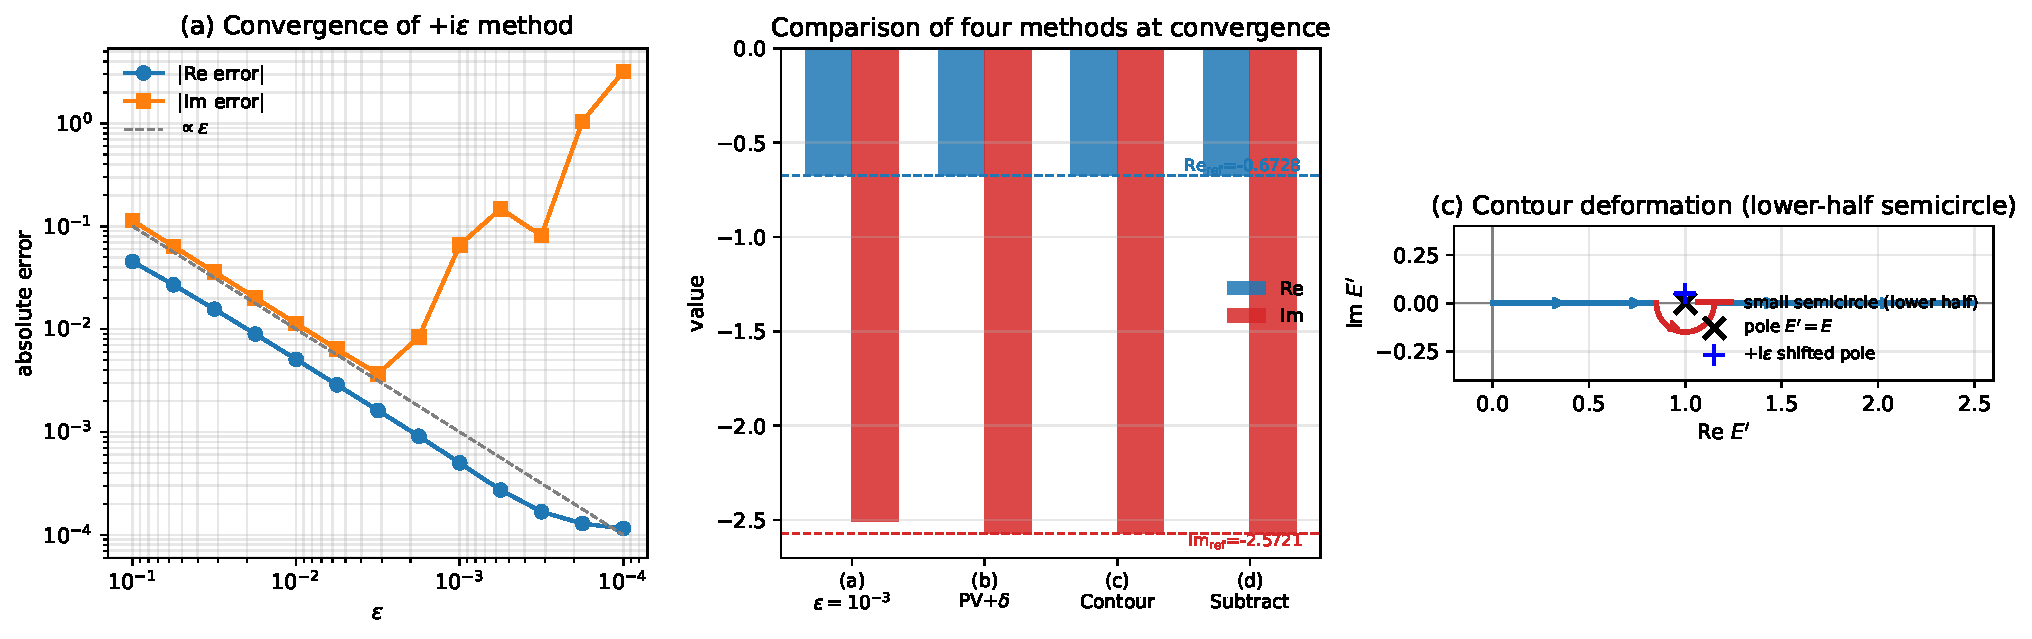
\includegraphics[width=0.98\linewidth]{ch07_pole_bypass}
    \caption{极点绕走的四种处理方式。
    左：方法 (a) 的绝对误差关于 $\epsilon$ 的扫描，
    实部误差 $\propto\epsilon^2$ (Lorentzian 偏置经过对称积分相消后剩二阶)，
    虚部误差 $\propto\epsilon$ (Lorentzian 与 $\delta$ 的有限宽度差异).
    中：四种方法在 \emph{已收敛} 取值下的实部 / 虚部柱状对比，
    虚线为参考解 $\Re I=-0.6728$, $\Im I=-\pi f(E)\approx -2.5721$。
    方法 (b)(c)(d) 与参考值的差异已在 $10^{-7}$ 量级内 (求积本身的离散误差)。
    右：方法 (c) 在复 $E'$-平面上的围道示意。
    极点 $E'=E$ 落在围道之外 (蓝色 $+\rmi\epsilon$ 移位极点亦如此)，
    下半圆贡献 $-\rmi\pi f(E)$ 即 \eqref{eq:numexp-ch07-SP} 中的 $\delta$ 部分。}
    \label{fig:numexp-ch07}
\end{figure}

数值结果 (脚本输出)：
\begin{center}\small
\begin{tabular}{lcc}
\hline
方法 & $\Re I$ & $\Im I$ \\
\hline
参考解 (高精度自适应)             & $-0.67280067$ & $-2.57211852$ \\
(a) $+\rmi\epsilon$, $\epsilon=10^{-3}$ & $-0.67330$    & $-2.50637$    \\
(b) PV $+\delta$ 拆分              & $-0.67280067$ & $-2.57211852$ \\
(c) 围道形变 ($r=10^{-3}$)        & $-0.67280067$ & $-2.57211852$ \\
(d) 减法 $+$ 解析修正              & $-0.67280067$ & $-2.57211852$ \\
\hline
\end{tabular}
\end{center}

\subsection*{物理讨论}

\begin{itemize}
  \item \textbf{(a) 的本质是磨平 (regularization).}
        把 $\delta$-函数换成宽度 $\epsilon$ 的 Lorentzian
        $\frac{1}{\pi}\frac{\epsilon}{(E-E')^2+\epsilon^2}$；要逼近 $\delta$ 必须 $\epsilon\to 0$，
        但同时积分网格也必须比 $\epsilon$ 更细才能分辨 Lorentzian 峰，
        因此实践上需要 $\epsilon\,\Delta E^{-1}\gtrsim 10$，
        而 $\Im$ 误差仍只能以 $\epsilon$ 一阶下降。
        $+\rmi\epsilon$ 在\emph{形式推导} 中无可替代，
        但若直接用作数值方案则收敛缓慢。
  \item \textbf{(b) 是教科书做法。}
        把奇异性\emph{解析地} 处理掉之后，
        余下的被积函数完全光滑，求积可以达到机器精度。
        代价是要求被积权重 $f(E')$ 在极点处可微 (取 $f(E')-f(E)$)。
  \item \textbf{(c) 给出 $+\rmi\epsilon$ 处方的几何意义。}
        $+\rmi\epsilon$ 把极点抬到上半平面等价于把围道压到下半平面。
        在与时间有关的描述中 (cf.\ 第 \ref{ch:Smat1P}, \ref{ch:cross} 章)，
        $+\rmi 0^+$ 选取的正是\emph{出射} ($t\to+\infty$) 边界条件：
        极点的小虚部对应于\emph{衰减的入射波尾}, $\rme^{-\epsilon t}$，
        把因果性翻译成围道方向的具体规则。
        这是 $G^+$ vs $G^-$ 二分法在数值层面的几何呈现。
  \item \textbf{(d) 是色散关系的"主力".}
        在第 \ref{ch:analytic} 章我们要从 $\Im T(E)$ 的实验测量
        重构 $\Re T(E)$ (Kramers--Kronig / forward dispersion)：
        实部恰好是 \eqref{eq:numexp-ch07-main} 的形式。
        减法做得更进一步、可以取多次减除以保证大 $E'$ 收敛，
        是高能物理 / 核物理 / 光学色散分析的标准操作。
\end{itemize}

四种方法对同一物理量给出一致的数值，
彼此互相充当交叉验证；
\eqref{eq:Gpm-def} 中的 $\pm\rmi 0^+$ 不再是符号上的"小修饰"，
而是\emph{有具体可计算后果} 的物理边界条件。
